%%%%%%%%%%%%%%%%%%%%%%%%%%%%%%%%%%%%%%%%%%%%%%%%%%%%%%%%%%%%%%%%
%%%%%%%%%%%%%%%%%%%%%%%%%%%%%%%%%%%%%%%%%%%%%%%%%%%%%%%%%%%%%%%%
%%%%
%%%% This text file is part of the source of 
%%%% `Introduction to High-Performance Scientific Computing'
%%%% by Victor Eijkhout, copyright 2012-2022
%%%%
%%%% This book is distributed under a Creative Commons Attribution 3.0
%%%% Unported (CC BY 3.0) license and made possible by funding from
%%%% The Saylor Foundation \url{http://www.saylor.org}.
%%%%
%%%% hpc_course.tex : main file for the big HPC slide deck
%%%%
%%%%%%%%%%%%%%%%%%%%%%%%%%%%%%%%%%%%%%%%%%%%%%%%%%%%%%%%%%%%%%%%
%%%%%%%%%%%%%%%%%%%%%%%%%%%%%%%%%%%%%%%%%%%%%%%%%%%%%%%%%%%%%%%%

\documentclass[11pt,headernav]{beamer}

\usepackage{beamerthemeTACC}
\parskip=.5\baselineskip plus .5\baselineskip
\input semester

\setcounter{tocdepth}{1}
\AtBeginSection[]
{
  \begin{numberedframe}
    \frametitle{Table of Contents}
    \tableofcontents[currentsection]
  \end{numberedframe}
}

\usepackage{pslatex}
\usepackage{amsmath,comment,multirow,multicol} %% ,arydshln

\setbeamertemplate{footline}{Eijkhout: programming}

\newdimen\unitindent \unitindent=20pt

\usepackage{comment}

\input slidemacs
\input snippetmacs
\input scimacs

\usepackage{makeidx}
\makeindex

\includecomment{diagonalstorage}

\begin{document}
\parskip=10pt plus 5pt minus 3pt

\title{HPC tools for programming}
\author{Victor Eijkhout}
\date{2022}

\begin{frame}{}
  \titlepage
\end{frame}

%% \begin{numberedframe}{Contents}
%%   \tableofcontents
%% \end{numberedframe}

\begin{numberedframe}{Justification}

  High Performance Computing requires,
  beyond simple use of a programming language,
  a~number programming tools. These tutorials
  will introduce you to some of the more important ones.

\end{numberedframe}

\Level 0 {Intro to file types}

\begin{numberedframe}{File types}
  \label{sl-tut:file-type}
  \begin{tabular}{ll}
    \toprule
    \multicolumn{2}{c}{Text files}\\
    \midrule
    Source&Program text that you write\\
    Header&also written by you, but not really program text.\\
    \midrule
    \multicolumn{2}{c}{Binary files}\\
    \midrule
    Object file&The compiled result of a single source file\\
    Library&Multiple object files bundled together\\
    Executable&Binary file that can be invoked as a command\\
    Data files&Written and read by a program\\
    \bottomrule
  \end{tabular}
\end{numberedframe}

\begin{numberedframe}{Text files}
  \label{sl-tut:text-file}
  \begin{itemize}
  \item Source files and headers
  \item You write them: \emph{make sure you master an editor}
  \item The computer has no idea what these mean.
  \item They get compiled into programs.
  \end{itemize}
  (Also `just text' files: READMEs and such)
\end{numberedframe}

\begin{numberedframe}{Binary files}
  \label{sl-tut:bin-file}
  \begin{itemize}
  \item Programs. (Also: object and library files.)
  \item Produced by a compiler. 
  \item Unreadable by you; executable by the computer.
  \end{itemize}
  Also binary data files; usually specific to a program.\\
  (Why don't programs write out their data in readable form?)
\end{numberedframe}

\Level 0 {Compilation}

\begin{numberedframe}{Compilers}
  Compilers: a major CS success story.
  \begin{itemize}
  \item The first Fortran compiler (Backus, IBM, 1954):\\
    multiple man-years.
  \item These days: semester project for graduate students.\\
    Many tools available (\n{lex}, \n{yacc}, \n{clang-tidy})\\
    Standard textbooks (`Dragon book')
  \item Compilers are very clever!\\
    You can be a little more clever in assembly --~maybe\\
    but compiled languages are $10\times$ more productive.
  \end{itemize}
\end{numberedframe}

\begin{numberedframe}{Compilation vs interpreted}
  \begin{itemize}
  \item Interpreted languages: lines of code are compiled `just-in-time'.\\
    Very flexible, sometimes very slow.
  \item Compiled languages: code is compiled to machine language:\\
    less flexible, very fast execution.
  \item Virtual machine: languages get compiled to an intermediate language\\
    (Pascal, Python, Java)\\
    pro: portable; con: does not play nice with other languages.
  \item Scientific computing languages:
    \begin{itemize}
    \item Fortran: pretty elegant, great at array manipulation\\
      Note: Fortran20003 is modern; F77 and F90 are not so great.
    \item C: low level, allows great control, tricky to use
    \item C++: allows much control, more protection, more tools\\
      (kinda sucks at arrays)
    \end{itemize}
  \end{itemize}
\end{numberedframe}

\begin{numberedframe}{Simple compilation}
  \label{sl-tut:compile1}
  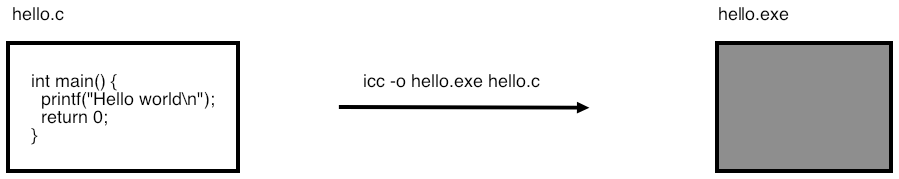
\includegraphics[scale=.3]{compilelink1}
  \begin{itemize}
  \item From source straight to program.
  \item Use this only for short programs.
  \end{itemize}
  \begin{multicols}{2}
    \small
\begin{verbatim}
  %% gcc hello.c
  %% ./a.out
  hello world
\end{verbatim}
\columnbreak
\begin{verbatim}
%% gcc -o helloprog hello.c
%% ./helloprog
hello world
\end{verbatim}
  \end{multicols}
\end{numberedframe}

\begin{numberedframe}{Exercise 1, C++ version}
  Create a file with these contents, and make sure you can compile it:
  
  \strippedinput{../code/compilecxx}{hello.cxx}
\end{numberedframe}

\begin{numberedframe}{Exercise 1, C version}
  Create a file with these contents, and make sure you can compile it:
  
  \strippedinput{../code/compilec}{hello.c}
\end{numberedframe}

\begin{numberedframe}{Separate compilation}
  \label{sl-tut:compile2}
  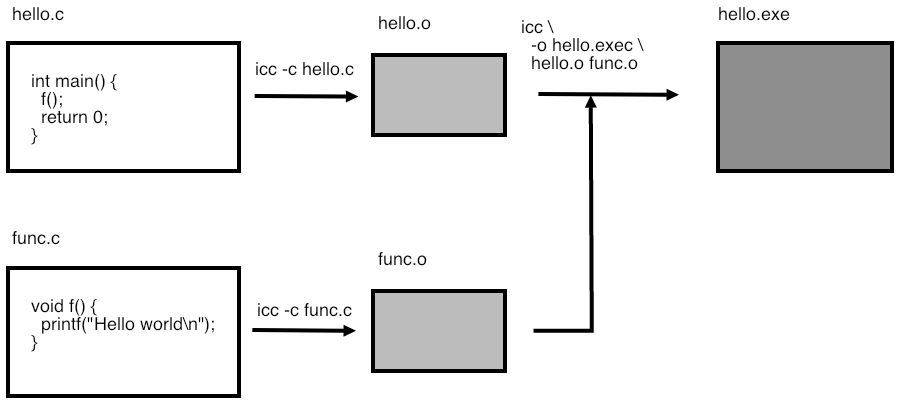
\includegraphics[scale=.3]{compilelink2}
  \begin{itemize}
  \item Large programs best broken into small files,
  \item \ldots~and compiled separately (can you guess why?)
  \item Then `linked' into a program; linker is usually the same as the compiler.
  \end{itemize}
\end{numberedframe}

\begin{numberedframe}{Exercise 2, C++ version}
  \label{sl-tut:compile3cxx}
\begingroup \footnotesize
Make the following files:
\begin{multicols}{2}
  Main program: \n{fooprog.cxx}
  \strippedinput{../code/compilecxx}{fooprog.cxx}
  \columnbreak
  Subprogram: \n{foosub.cxx}
  \strippedinput{../code/compilecxx}{foosub.cxx}
\end{multicols}
\endgroup
\end{numberedframe}

\begin{numberedframe}{Exercise 2, C version}
  \label{sl-tut:compile3c}
\begingroup \footnotesize
Make the following files:
\begin{multicols}{2}
  Main program: \n{fooprog.c}
  \strippedinput{../code/compilec}{fooprog.c}
  \columnbreak
  Subprogram: \n{foosub.c}
  \strippedinput{../code/compilec}{foosub.c}
\end{multicols}
\endgroup
\end{numberedframe}

\begin{numberedframe}{Exercise 2 continued, C++ version}
  \begin{itemize}
  \item Compile in one:
\begin{verbatim}
icpc -o program fooprog.cxx foosub.cxx
\end{verbatim}
\item Compile in steps:
\begin{verbatim}
icpc -c fooprog.cxx
icpc -c foosub.cxx
icpc -o program fooprog.o foosub.o
\end{verbatim}
What files are being produced each time?
  \end{itemize}
Can you write a shell script to automate this?  
\end{numberedframe}

\begin{numberedframe}{Exercise 2 continued, C version}
  \begin{itemize}
  \item Compile in one:
\begin{verbatim}
icc -o program fooprog.c foosub.c
\end{verbatim}
\item Compile in steps:
\begin{verbatim}
icc -c fooprog.c
icc -c foosub.c
icc -o program fooprog.o foosub.o
\end{verbatim}
What files are being produced each time?
  \end{itemize}
Can you write a shell script to automate this?  
\end{numberedframe}

\begin{numberedframe}{Header files}
  \begin{itemize}
  \item
    \n{extern} is not the best way of dealing with `external references'
  \item Instead, make a header file \n{foo.h} that only contains
\begin{lstlisting}
void bar(char*);
\end{lstlisting}
\item Include it in both source files:
\begin{lstlisting}
#include "foo.h"
\end{lstlisting}
\item Do the separate compilation calls again.
  \end{itemize}
  Now is a good time to learn about makefiles~\ldots
\end{numberedframe}

\begin{numberedframe}{Compiler options 101}
  \label{sl-tut:option1}
  \begin{itemize}
  \item You have just seen two compiler options.
  \item Commandlines look like
\begin{verbatim}
command [ options ] [ argument ]
\end{verbatim}
where square brackets mean: `optional'
\item Some options have an argument
\begin{verbatim}
icc -o myprogram mysource.c
\end{verbatim}
\item Some options do not.
\begin{verbatim}
icc -g -o myprogram mysource.c
\end{verbatim}
\item Question: does \n{-c} have an argument? How can you find out?
\begin{verbatim}
icc -g -c mysource.c
\end{verbatim}
  \end{itemize}
\end{numberedframe}

\begin{numberedframe}{Object files}
  \label{sl-tut:object}
  \begin{itemize}
  \item Object files are unreable. (Try it. How do you normally view files?
    Which tool sort of works?)
  \item But you can get some information about them.
  \end{itemize}
  \begin{multicols}{2}
    \small
\begin{verbatim}
  #include <stdlib.h>
  #include <stdio.h>
  void bar(char *s) {
    printf("%s",s);
  }
\end{verbatim}
\columnbreak
\begin{verbatim}
  [c:264] nm foosub.o
  0000000000000000 T _bar
  U _printf
\end{verbatim}
 Where \n{T}: stuff defined in this file\\
  \n{U}: stuff used in this file
  \end{multicols}
\end{numberedframe}

\begin{numberedframe}{Compiler options 102}
  \label{sl-tut:options2}
  \begin{itemize}
  \item Optimization level: \n{-O0}, \n{-O1}, \n{-O2}, \n{-O3}\\
    (`I~compiled my program with oh-two')\\
    Higher levels usually give faster code. Level~3 can be unsafe. (Why?)
  \item \n{-g} is needed to run your code in a debugger. Always include this.
  \item The ultimate source is the `man page' for your compiler.
  \end{itemize}
\end{numberedframe}

\begin{numberedframe}{Compiler optimizations}
\begin{multicols}{2}
  Common subexpression elimination:
\begin{lstlisting}
x1 = pow(5.2,3.4) * 1;    
x2 = pow(5.2,3.4) * 2;
\end{lstlisting}
  becomes
\begin{lstlisting}
t = pow(5.2,3.4);
x1 = t * 1;    
x2 = t * 2;
\end{lstlisting}
\columnbreak
Loop invariants lifting
\begin{lstlisting}
for (int i=0; i<1000; i++)
  s += 4*atan(1.0) / i;
\end{lstlisting}
becomes
\begin{lstlisting}
t = 4*atan(1.0);
for (int i=0; i<1000; i++)
  s += t / i;
\end{lstlisting}
\end{multicols}
\end{numberedframe}

\begin{numberedframe}{Example of optimization}
  Givens program
\cxxverbatimsnippet{givensfunx}
Run with optimization level 0,1,2,3 we get:
\begin{verbatim}
Done after 8.649492e-02
Done after 2.650118e-02
Done after 5.869865e-04
Done after 6.787777e-04
\end{verbatim}
\end{numberedframe}

\begin{numberedframe}{Exercise 3}
  \label{sl:ex:rotate}
  The file \n{rotate.cxx} (or \n{rotate.c})
  can be speeded up by compiler transformations.\\
  Compile this file with optimization levels \n{0,1,2,3}\\
  (try both the Intel and gcc compilers)\\
  observe run time and conjecture what transformations can explain this.
  
  Apply these transformations by hand and see if they indeed
  lead to improvements.
  
  Write a report of your investigations.
\end{numberedframe}

\Level 0 {Libraries}

\begin{numberedframe}{Libraries}
  \label{sl-tut:}
  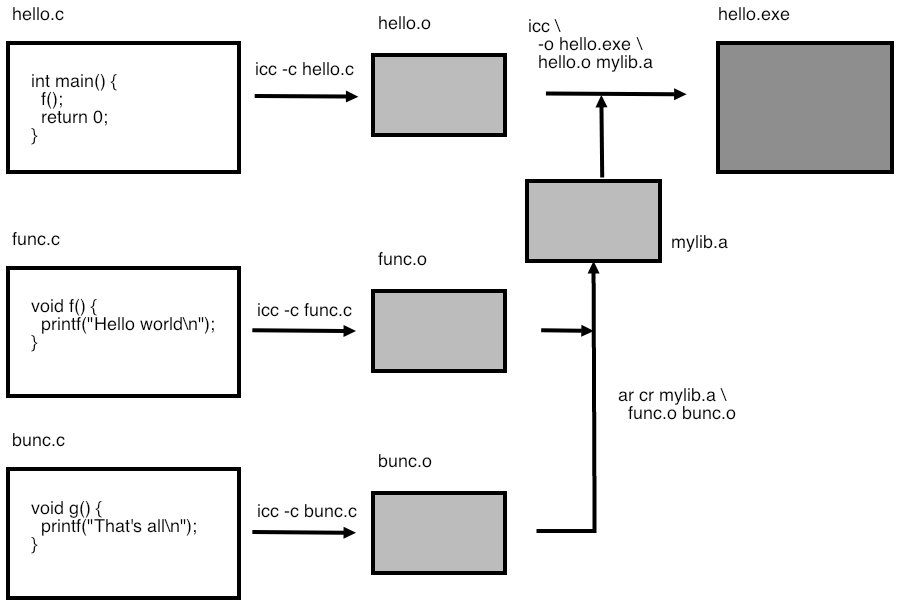
\includegraphics[scale=.25]{compilelink3}
  \begin{itemize}
  \item Sometimes you have many object files:\\
    convenient to bundle them
  \item Easier to link to
  \item Easy to distribute as a product.
\item Software library: collection of object files that can be linked to a main program.
  \end{itemize}
\end{numberedframe}

\begin{numberedframe}{Static / non-shared libraries}
  \label{sl-tut:libar}
  \begin{itemize}
  \item Static libraries are created with \n{ar}
  \item Inspect them with \n{nm}
  \item Link as object file:
\begin{verbatim}
icc -o myprogram main.o ../lib/libfoo.a
\end{verbatim}
\item Or:
\begin{verbatim}
icc -o myprogram main.o -L../lib -lfoo.a
\end{verbatim}
  \end{itemize}
  \begin{multicols}{2}
    \small
\begin{verbatim}
mkdir ../lib
ar cr ../lib/libfoo.a foosub.o
\end{verbatim}
\columnbreak
\begin{verbatim}
%% nm ../lib/libfoo.a 

../lib/libfoo.a(foosub.o):
00000000 T _bar
         U _printf
\end{verbatim}
  \end{multicols}
\end{numberedframe}

\begin{numberedframe}{Static library example}
  \label{sl-tut:liba}
 Use \n{ar} to add object files to \n{.a} file.

\footnotesize
\begin{verbatim}
icc -g -O2 -std=c99 -c foosub.c
for o in foosub.o ; do \
  ar cr libs/libfoo.a ${o} ; \
done
icc  -o staticprogram fooprog.o -Llibs -lfoo
-rwx------ 1 eijkhout G-25072 38192 Sep 23 18:15 staticprogram
./staticprogram
hello world
\end{verbatim}
\end{numberedframe}

\begin{numberedframe}{Dynamic/shared libraries}
  \label{sl-tut:libso.1}
  Created with the compiler,\\
  \n{-shared} flag.
\begin{verbatim}
icc -O2 -std=c99 -fPIC -c foosub.c
icc -o libs/libfoo.so -shared foosub.o
icc -o dynamicprogram fooprog.o -Llibs -lfoo
\end{verbatim}
\end{numberedframe}

\begin{numberedframe}{Executable size}
  \label{sl-tut:exsize}
  Static libraries are baked into the executable\\
  shared libraries are linked at runtime.

  \footnotesize
\begin{verbatim}
# Making static library
icc  -o staticprogram fooprog.o -Llibs -lfoo
-rwx------ 1 eijkhout G-25072 28232 Sep 23 14:25 staticprogram
# Using dynamic library
icc -o dynamicprogram fooprog.o -Llibs -lfoo
-rwx------ 1 eijkhout G-25072 28160 Sep 23 14:25 dynamicprogram
\end{verbatim}
\begin{comment}
# Using shared library
icc -o rpathprogram fooprog.o -Wl,-rpath=./libs -Llibs -lfoo
-rwx------ 1 eijkhout G-25072 28160 Sep 23 14:25 rpathprogram
\end{comment}
\end{numberedframe}

\begin{numberedframe}{Needs something more}
  \label{sl-tut:libso.3}
  Program can not immediately be run.\\
  Use \n{ldd} to see what libraries it needs:

  \footnotesize
\begin{verbatim}
./dynamicprogram: error while loading shared libraries:
      libfoo.so: cannot open shared object file: No such file or directory

ldd dynamicprogram | grep libfoo
        libfoo.so => not found
\end{verbatim}
\end{numberedframe}

\begin{numberedframe}{The ell-dee library path}
  \label{sl-tut:libso.4}
Libraries are found by updating the \n{LD_LIBRARY_PATH}:

  \footnotesize
\begin{verbatim}
export LD_LIBRARY_PATH=${LD_LIBRARY_PATH}:./libs
ldd dynamicprogram | grep libfoo
        libfoo.so => ./libs/libfoo.so (0x00002ad6604c1000)
./libs dynamicprogram
hello world
\end{verbatim}
\end{numberedframe}

\begin{numberedframe}{The rpath}
  \label{sl-tut:libso.5}
  You can also bake the path into the program:

  \footnotesize
\begin{verbatim}
icc -O2 -std=c99 -fPIC -c foosub.c
icc -o libs/libfoo.so -shared foosub.o
icc -o rpathprogram fooprog.o \
    -Wl,-rpath=./libs -Llibs -lfoo
-rwx------ 1 eijkhout G-25072 28160 Sep 23 13:41 rpathprogram
./rpathprogram
hello world
\end{verbatim}
(Notice the bizarre combination of minuses and commas)
\end{numberedframe}

\end{document}

\Level 0 {Cross-language linking}

\begin{numberedframe}{}
  \label{sl-tut:}
  \begin{itemize}
  \item 
  \end{itemize}
\end{numberedframe}

\begin{numberedframe}{}
  \label{sl-tut:}
  \begin{itemize}
  \item 
  \end{itemize}
\end{numberedframe}

